
\hspace{1.5cm}2021 marked the 80th anniversary of the invention of modern computer technology, an industry that has grown exponentially since then and has been a great help. Certainly, the human brain also has its limits, yet many try to understand things that cannot be achieved with conventional thinking. Sometimes it is even impossible to understand what lies behind a complex process, but as with the invention of computer technology, machine learning opens a multitude of doors that need to be opened, not understood.\\ 


\section{Introduction to Machine Learning}
Machine learning (ML) is nothing but a powerful tool with an unimaginable range of applications. Not only is it used in everyday life for seemingly difficult tasks, but every day new applications are found and explored that are enormous. In this case, despite the tremendous advances in software optimisation, simulating a complex biological environment is a difficult and, more importantly, expensive task that still has a ways to go. These types of problems are the focus of machine learning because it uses an alternative approach. Instead of tackling  the problem in the profound sense, ML aims to collect data and fill in the gaps to optimise the prediction error. This is very useful because the underlying understanding of the process is not required for the prediction to turn out pretty well, and in many cases, better. This is fascinating. As mentioned earlier, the main role of ML is to optimise problems, but for this to happen, some conditions must be met.\\

We humans need some kind of experience to learn, and patterns are used to build behaviours that we think are best for the situation onward.
Machine learning is somehow similar, a \textbf{dataset}, which would be analogous to experience, consists of \textbf{features} or attributes of each situation. There are two types of features:
\begin{itemize}
    \item \textbf{Response features}  are the features for which we want the model make predictions. For this to happen, some other features' information which may give us hints on how to solve the problem is required. These features need to be linked to the response features somehow, and hand out valuable information.
    
    
    \item \textbf{Descriptors} are the kind of features which set up the context surrounding the response features. Therefore, they need to have to do with the response features. The better the link between descriptors and response features, the better the prediction.

\end{itemize}
\vspace{0.6cm}

Using these attributes, algorithms can be trained minimising the error between the response variable estimations and the actual observations. They can shape models which best adequate to every possible situation; the bigger the dataset and the more the information in the features, the more accurate the model built by the algorithm. Algorithms themselves are optimisable functions with their own \textbf{hyperparameters} that can be tuned according to the context. There are many times of algorithms, from \textbf{regressors}, algorithms for which the response variable is continuous; \textbf{classifiers}, for which the response feature is discrete; to \textbf{clustering algorithms}, which do not need a response variable.\\

Regressors and classifiers can also be more simple or more complex; algorithms which build linear model are considered the most simple, while non linear model building algorithms or even ensemble methods (methods which use up more than one algorithm at once) are considered more complex. Sometimes, a simple one is enough to build a reliable model; in this case, it will be demonstrated a complex one better approximates to the situation of this burdensome biological problem.

\section{Machine Learning Algorithms}
To better understand the world of machine learning, we need to describe the underlying algorithms, and a few examples will make it clearer how it works.
\subsection{Linear Regression}
Among the algorithms of ML, the linear regression algorithm is the simplest of all and the easiest to understand. 
A linear regression algorithm aims to learn a function that makes predictions for the response variable by a linear combination of the input variables (or descriptors) \cite{Zhou21a}, that is, having an input vector $X=(x_1,x_2,x_3,...,x_M)$ corresponding to the $M$ descriptor features, the form of the estimation is:
\begin{equation}
\label{eqn:f(X)}
    f(X)=\beta_0+\sum_{i=1}^M\beta_ix_i,
\end{equation}
where $\beta=(\beta_0,\beta_1,...,\beta_M)$ are the coefficients linked to $(1,X)$, and $f(X)$, the response variable estimation.

To calculate the optimal coefficients that best predict the outcome, the $least$ $squares$ method is usually used. Here, the residual sum of squares (RSS) is defined as the loss (or cost) function, $i.e.$, the function to be minimised:
\begin{equation}
\label{eqn:RSS}
RSS(\beta)=\sum_{i=1}^N(y_i-\hat{y}_i)^2.
\end{equation}
where N is the number of observations; $\hat{y_i}$ is the estimate of each observation, or put another way, $\hat{y_i}=f(\textbf{X}_i)$, where \textbf{X} is the N x M matrix of descriptors/observations corresponding to the dataset; and $y_i$ is the actual value of the response feature for each observation column $\textbf{X}_i$.

After a little algebra (attached demonstration in appendix), the $\beta$ that best fits the model is as follows:
\begin{equation}
    \beta=(\textbf{X}^T\textbf{X})^{-1}\textbf{X}^T\textbf{y}
\end{equation}
where $\textbf{y}=(y_1,y_2,...,y_N)$. Then $f(X)$ can be properly addressed using equation \ref{eqn:f(X)}.
 
\subsubsection{Ridge}
In ridge regression, a regularisation parameter\footnote{A regularisation parameter is usually used to avoid overfitting the model. By setting the RSS with this regularisation parameter, the coefficients in the variables are penalised, so there is a chance to make a leaner or tighter prediction depending on whether the model is sufficiently constrained on the training data and whether it performs well on the raw data.} is attached to the previous RSS, which is minimised. As a result, the new RSS looks like this:
\begin{equation}
    RSS(\beta_{ridge})=\sum_{i=1}^N(y_i-\hat{y}_i)^2+\alpha \sum_{i=1}^M\beta_i^2,
\end{equation}
where $\alpha(>0)$ is a tuning parameter, so it can be changed to get a better prediction.

This linear regressor is a better option as it adapts to the context and the problem better and is a choice which (when $\alpha$=0) can implement  the simple linear regression explained earlier.\\

Ridge regression is defined in the procedure below:

\begin{algorithm}[H]
\caption{Ridge Regression}
\begin{algorithmic}[1]
    \Require Training set $D = \{ (\textbf{X}_1, y_1), (\textbf{X}_2, y_2), . . . , (\textbf{X}_N, y_N)\}$;
    
    Regularisation parameter $\alpha$.
    \Ensure $f(X)$ regression function.
    
    \For{$i \gets 1$ to $N$}
    \State Define $\hat{y}_i$: \begin{equation}
        \hat{y}_i=f(\textbf{X}_i)=\beta_0+\sum_{i=1}^M\beta_i\textbf{X}_i
    \end{equation}
    
    \EndFor
    \State Find the new $\beta_{ridge}=(\textbf{X}^T\textbf{X} + \alpha \mathbb{1})^{-1}\textbf{X}^T\textbf{y}$ (demonstration in appendix) or: \begin{equation}
        \argmin_{\beta}\sum_{i=1}^N(y_i-\hat{y}_i)^2+\alpha \sum_{i=1}^M\beta_i^2
    \end{equation}
    \State Tune $\alpha$ for optimal results.
\end{algorithmic}
\end{algorithm}
\subsection{Tree-Based Methods}
Although linear regression may seem as a powerful candidate, when it comes to describing such complex processes as the changes in conformations in proteins, it will be demonstrated more complex yet more computationally expensive methods are needed. For this, Random Forest is huge candidate. Random Forest is a nonlinear ensemble algorithm from the family of tree-based methods that implements the decision tree algorithm multiple times (hence the Forest designation). It has proven to be a viable candidate in many biological problems such as gene expression \cite{geneexpression} and damage localisation \cite{DNAdamage}, protein ligand residue recognising \cite{bindingresidues} or even closer, for many protein structure prediction techniques \cite{KALAISELVI2020107885}.

Lets firstly start by defining the components of this Random Forest algorithm, decision trees.
\subsubsection{Decision Trees}
Decision trees build regression (or classification) models using a tree structure. The dataset is optimally partitioned among features so that a decision can be made. Each of these resting datasets is called a node, and they represent the different levels of this decision tree. A representative illustration of a decision tree is Figure 2.1, which can serve as a guide.\\

A root node containing all the data used in training the algorithm optimally splits into two datasets (parent node splits into two child nodes) according to a single feature. For this optimal split, the $squared$ $error$ criterion was used, looking for the split with the smallest mean squared error (Section 2.4.1). After each split, either a terminal node or a decision node can be the new node. Decision nodes are those that can be split further, while end nodes are those that are not able to further split. There are several ways to determine whether a node will be a decision or terminal node: the number of observations in the node, the layer of the algorithm (the maximum depth hyperparameter can be set), the variance in the node...\\\\

\begin{figure}[h!]
    \centering
    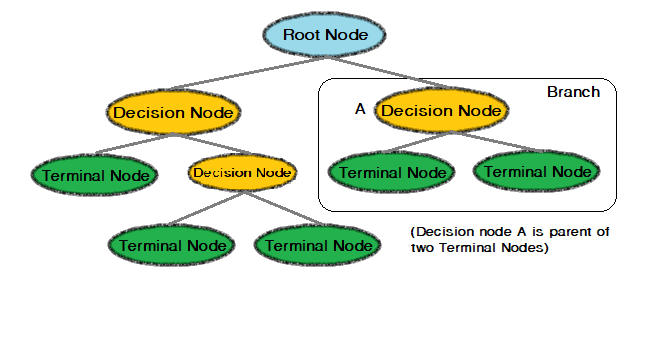
\includegraphics[width=0.85\textwidth]{Images/Methods/detreenodes.png}
    \caption{Visual Representation of a Decision Tree.}
\end{figure}
Each terminal node is assigned a response feature value, which is the mean value of the response feature of all observations in that cluster. The goal of decision trees, as with any regressor, is to predict the response feature value for new data containing descriptor information. After the new data point has passed through the decision trees, it is assigned the response feature value of the terminal node at which it arrived.\\\\ 
The algorithm for decision tree learning is on the next page.
\begin{algorithm}[H]
\caption{Decision Tree Learning}
\begin{algorithmic}[1]
    \Require Training set $D = \{ (\textbf{X}_1, y_1), (\textbf{X}_2, y_2), . . . , (\textbf{X}_M, y_M)\}$;
    
    Feature set $A = \{a_1, a_2,..., a_N\}$.
    
    
    
    \Ensure A decision tree with root node $i$.
    
    \hspace{-1.5cm}\textbf{Process:} Function Tree($D, A$)
    
    \State Generate node $i$.
    \If {All samples in $D$ belong to the same class $C$}
    
    \State Mark node $i$ as a class $C$ terminal node; {\Return}
    \EndIf
    \If {$A =\{\emptyset\}$ \Or all samples in $D$ take the same value on $A$}
    
    \State Mark node $i$ as a terminal node, and its class label is the majority 
    
    class in $D_i$; {\Return}
    \EndIf
    
    \State Select the optimal splitting feature $a_*$ from $A$
    
    \For{each value $a_*^\nu$ in $a_*$}
    
    \State Generate a branch for node $i$; Let $D_v$ be the subset of samples
    
    taking value $a_*^v$ on $a_*$;
    
    \If{$D_\nu$ is empty} 
    
    \State Mark this child node as a terminal node, and label it with the 
    
    \hspace{0.65cm}majority class in $D$; {\Return}
    \Else
    
    \State Use Tree($D_v , A \backslash \{a_*\}$) as the child node.
    
    \EndIf
    \EndFor
    
\end{algorithmic}
\end{algorithm}
\hspace{14cm}\cite{Zhou21a}\\






\subsubsection{Random Forest}
Random Forest (RF) is a decision tree founded algorithm whose idea is to merge various trees
through the idea of ensemble learning. There is no union linking each decision tree, but each and every decision tree in the forest shape the
final product (or output) of this model. 
In a regression problem, the average output of the individual decision trees is the final result \cite{YUAN2022100026}.\\

The feature sample for the decision trees in the Random Forest is chosen arbitrarily, they sample without replacement. This means, when a set of features needs to be determined for each decision tree, this is carried out randomly, and as well as more than one decision tree being able to contain the same feature, the same feature can appear twice in each decision tree (bootstrapping in Section 2.5.3).\\

As it can be observed in Figure 2.2, each decision tree is usually different, as it consists of distinct feature organisations, and as the input travels through each decision tree, it gets a response feature value. All this values are merged in a mean to get the final output. 
\begin{figure}[h!]
    \centering
    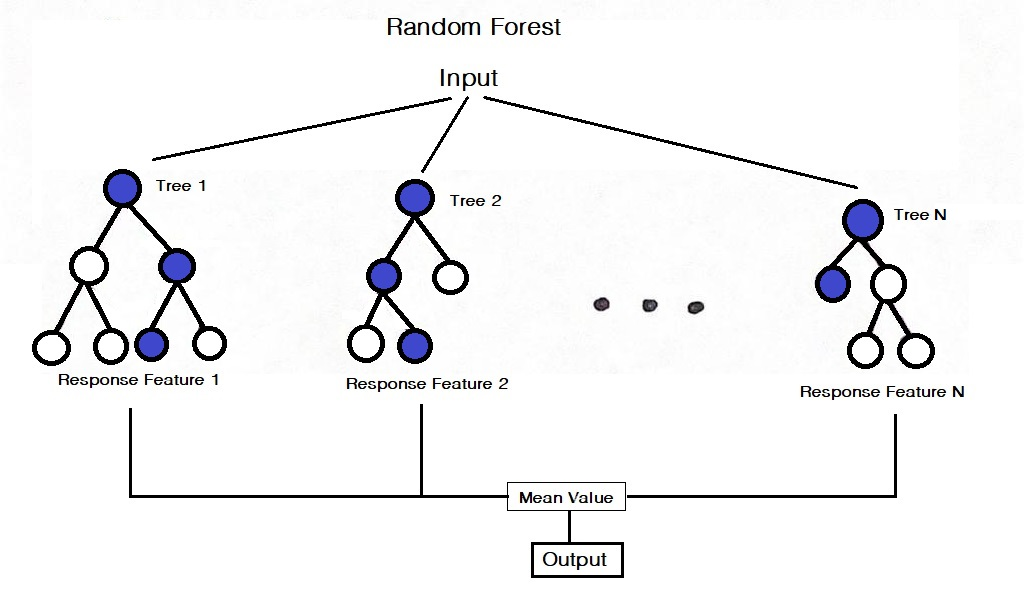
\includegraphics[width=0.8\textwidth]{Images/Methods/RFout.jpeg}
    \caption{A Random Forest simplified diagram. The input descriptor data travels through N decision trees where the blue nodes represent the decisions taken in every split. The mean is taken of every response feature value.}
\end{figure} 
\subsection{Clustering Algorithms}
When talking about machine learning algorithms, clustering algorithms are a big part of what is called $unsupervised$ $learning$ in the machine learning culture. These algorithms, as the name itself remarks, do not require tags or response variables of any sort, as they are programmed to find patterns in the raw data. Clustering algorithms classify the data into different groups, taking into account similarities, and they can be very useful in sorting molecules or even descriptors themselves by taking into account the correlation between them.

\subsubsection{K-means Clustering}

K-means is a widely known clustering method, the simplest and in many cases the most useful. In k-means, n observations are clustered into a number of k clusters. The criterion used to determine whether an observation belongs to one cluster or another is the minimum distance\footnote{The distance described in these clustering algorithms refers to the p-dimensional euclidean distance in the descriptor space. For example, the distance between two observations a and b with 4 descriptors each $(x_1,x_2,x_3,x_4)$ is determined by:
\begin{equation}
    d(a,b)=\sqrt{\Delta x_1^2+\Delta x_2^2 + \Delta x_3^2 + \Delta x_4^2}
\end{equation}
where \Delta x_i=x_{ia}-x_{ib}.} to the mean of the descriptors of all the observations in every cluster, also known as the centroid.\\

The k-means algorithm works upon two principal steps, assignment and updating, which are iterated until convergence, when further iterations do not change the outcome of each and every cluster.\\\\

\begin{figure}[H]
    \centering
    \begin{subfigure}[H]{0.2\textwidth}
        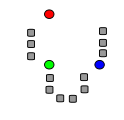
\includegraphics[width=\textwidth]{Images/Methods/K-means/K_Means_Example_Step_1.png}
        \vspace{-20pt}
        \caption{To initialise k-means, k (k=3 in this case) different cluster centroid points need to be randomly set.}
    \end{subfigure}
    \quad
    \begin{subfigure}[H]{0.2\textwidth}
        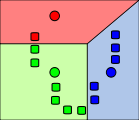
\includegraphics[width=\textwidth]{Images/Methods/K-means/K_Means_Example_Step_2.png}
        \vspace{1pt}
        \caption{Then, the observations need to be assigned to the cluster whose centroid is closer to it, therefore the $assignment$ $step$.}
    \end{subfigure}
    \quad
    \begin{subfigure}[H]{0.2\textwidth}
        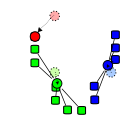
\includegraphics[width=\textwidth]{Images/Methods/K-means/K_Means_Example_Step_3.png}
        \vspace{-10pt}
        \caption{After the assignment is done, the mean of the observations in each cluster is set to be the new centroid of the cluster, the $update$ $step$.}
    \end{subfigure}
    \quad
    \begin{subfigure}[H]{0.2\textwidth} 
        \vspace{-40pt}
        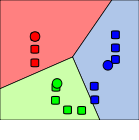
\includegraphics[width=\textwidth]{Images/Methods/K-means/K_Means_Example_Step_4.png}
        \vspace{-15pt}
        \caption{With the new centroids, the assignment step is again taken.}
    \end{subfigure}
    \caption{K-means clustering representation. This process is repeated until every centroid remains constant. Images from $Wikipedia$: $https://en.wikipedia.org/wiki/K$-$means\_clustering$. \\}
\end{figure}
The selection of the number of clusters is usually done by hand, but a good method to find out which k fits the model best is the $elbow$ $method$. 
The loss function is calculated for a varying number of clusters, and by plotting the result for each number of clusters, the goal is to look at the graph and find a vertex (the elbow). The $elbow$ represents a point at which further clustering does not significantly improve performance because the cost function decreases more slowly. In the next example (Figure 2.4), k-means was applied for different k values.
\begin{figure}[h!]
    \centering
    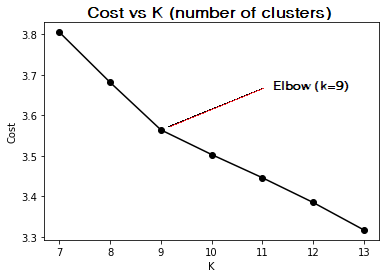
\includegraphics[scale=0.7]{Images/Methods/K-means/Fingerprints_elbow.png}
    \caption{Plotted cost function as a function of k. A clear elbow is found at k=9.}
\end{figure}


\subsubsection{Hierarchical Clustering}
On the other hand, hierarchical clustering is another approach that does not require the number of clusters to be fixed. Moreover, it is a very visual algorithm that provides a dendrogram, a "tree diagram showing taxonomic relationships". Here we explain the most common type of hierarchical clustering, agglomerative clustering. In this case, the dendrogram is built from the bottom up, starting with the single leafs up to the trunk \cite{James2013}.\\
 
Agglomerative clustering algorithms start with each observation forming a single cluster. N-1  times (in the case of N observations), the closest (most similar) pair of clusters is merged into a single cluster so that there is one less cluster at the next higher level. For this purpose, a distance measure between two clusters must be defined to set the criteria for merging them \cite{hastie01statisticallearning}. 

\begin{figure}[h]
    \centering
    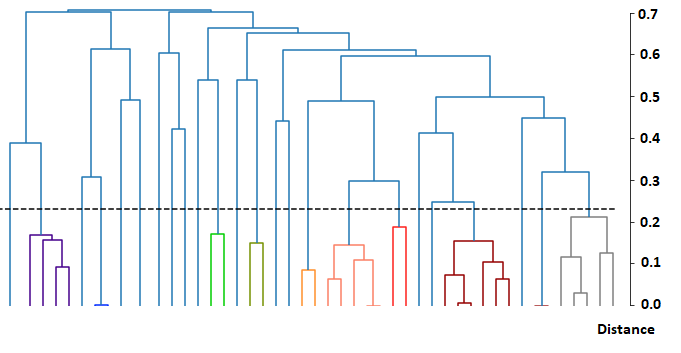
\includegraphics[scale=0.8]{Images/Methods/Hierarchical/Hierarchical dendogram.png}
    \caption{Example dendrogram with cluster criterion set. Each colour represents a cluster.}
\end{figure}


In hierarchical clustering, there are different types of linkage that take into account the distance between clusters. Imagine we have two clusters, A and B. The distance or dissimilarity measure is determined by considering the observations in each cluster in different ways:

\begin{itemize}
    \item \textbf{Ward linkage}: The objective of the Ward linkage criterion is to minimise within cluster variance. Therefore, in Ward linkage hierarchical clustering, the distance between clusters is determined based on the amount of variance increase that the merging of adjacent clusters A and B would lead to \cite{ward}.
    \item \textbf{Single linkage}: In single linkage hierarchical clustering, the distance between clusters is determined by the minimum distance between points of neighbouring clusters A and B.
    $$
    \min \{ d(a, b): a \in A, b \in B \}.
    $$
    \item \textbf{Complete linkage}: In complete linkage hierarchical clustering, the distance between clusters is determined by the maximum distance between points of adjacent clusters A and B.
    $$
    \max \{ d(a, b): a \in A, b \in B \}.
    $$
    \item \textbf{Average linkage}: In average linkage hierarchical clustering, the distance between clusters is determined by the average distance between all points of adjacent clusters A and B. $|A|$ and $|B|$ correspond to the number of observations in each cluster.
    $$
    \frac {1}{|A|.|B|}\sum_{a \in A}\sum_{b \in B}d(a, b).
    $$
    \item \textbf{Centroid linkage}: In centroid linkage hierarchical clustering, the distance between clusters is determined by the distance between centroids of adjacent clusters A and B:
    $$|
    |c_{A} - c_{B}||,
    $$
    where $c_{A}$ and $c_{B}$ are the positions of centroids of clusters A and B, respectively.
\end{itemize}\hspace{15cm}\cite{hastie01statisticallearning}

\subsection{Feature Selection Algorithms}
The predictive performance of a model depends on the adequate management of features. When avoiding unnecessarily high correlations among features that are able to trigger multicollinearity\footnote{Multicollinearity is a phenomenon which occurs when one descriptor is linearly related to combinations of other descriptors in the dataset, and it can be therefore predicted.}, it comes to mind which features ought to be selected. In a problem with way too many variables, an efficient algorithm can come in handy when performing the reduction.
\subsubsection{Sequential Feature Selection}
One of the simplest feature selection algorithms is the sequential feature selection algorithm. This is a greedy algorithm, meaning that, at every step, it makes the locally optimal choice, without considering whether this locally optimal choice will generate the globally optimal result.

Given a model, as well as some metric $J$ we can use to evaluate the performance every feature for that model, such as its F score (Section 2.4.3) or the cross-validation score of the model, the sequential feature selection algorithm chooses the $k$ best features for that model by following the procedure outlined below.

\begin{algorithm}[H]
\caption{Forward Sequential Feature Selection}
\begin{algorithmic}[1]
    \Require Set of all features $A=\{a_1, \dots, a_N\}$;
    
    Evaluation metric $J$;
    
    Target size of feature subset $M$.
    \Ensure Subset of best performing features $Y=\{y_1, \dots, y_M \}$.
    \State Start with empty set: $Y=\{\emptyset\}$.
    \For{$k \gets 1$ to $M$}
        \State Select next best feature: \[y_k = \argmax_{a_i\notin Y}{J(Y\cup a_i)}\]
        \State Add that feature to the feature subset: $Y=Y\cup y_k$.
    \EndFor
\end{algorithmic}
\end{algorithm}

That is, at every step, the algorithm evaluates the performance of every feature, then adds the best performing one to the final feature subset. It then repeats this procedure with all remaining features, until the predefined number of features is reached.\\

This algorithm can also be run backwards, where instead of starting from an empty set, $Y=\{\emptyset\}$, we instead start with a set that contains all features, $Y=X$. Then, at every step, rather than adding a new feature to the set, we instead remove the worse performing feature from it.\\

Sequential feature selection has certain advantages, such as its simplicity and speed, which makes it quite useful in scenarios where performance is a concern. However, it does have the disadvantages that it does not necessarily find the best possible subset of features for our model, and that a predefined number of features has to be chosen.


\section{PCA and Standardisation}
Also, whenever a large set of correlated variables has to be handled, principal components serve to summarise this group with a smaller number of representative variables that reflect all the variance of the original set of data on the whole. Principal components analysis (PCA) focuses on the method of calculating the principal components and the subsequent use of these components to understand the data. In addition to this, PCA also serves as a data visualisation tool, reducing the dimensionality of the data. It can also be used as a tool for data mapping, i.e. to fill in missing values in a data matrix. The issue is that each of the n observations occupies a p-dimensional space, but not all of these dimensions are of equal interest. PCA aims to find a small number of as interesting dimensions as possible, where the sense of interesting is determined by the degree of variance of the observations across each given dimension. Each of the dimensions found by PCA is a linear composition of the p features.\\

To perform PCA, variables must be centred and have a mean of zero. In addition, the results of PCA also depend on whether the variables have been scaled individually (each multiplied by a different constant). Since it is not advisable for the derived principal components to be based on an arbitrary choice of scaling, each variable is usually scaled so that it has a standard deviation of one before PCA is performed \cite{James2013}. 




\section{Evaluation Metrics}
Once the features are conditioned and established, it is time to properly evaluate each model and the content that corresponds to it, either to proceed with training or to evaluate the final version of the model itself.\\

For this, regression and correlation metrics are defined, as well as the feature evaluation metrics. 

\subsection{Regression Metrics}
Regression metrics are those that evaluate the performance of the algorithm, and are sometimes used by the algorithm itself to find the best possible version that is subsequently output.
Different regression metrics and algorithms that implement it are trying to solve different problems with distinct objectives. Each of these regression metrics are to be used most efficiently in the indicated cases, so the context needs to be taken into account. 
\subsubsection{Mean Absolute Error}
The mean absolute error (MAE) is defined by the sum of subtracting all the ``regressionwise" obtained values $\hat{y}_i$ from the real values $y_i$, and dividing the result by the number of observations $N$. Sometimes, a small change in an experiment can alter the result in a huge way, giving very wrong observations. While the rest of the data is still useful, estimations can be thrown off because of these observations. This regression metric is known for being keen with outliers (compared to the ones discussed later on), this means, it is apt to use in a datasets with possible mistakes and where the data may wrongly deviate. MAE is defined by the following formula:
\begin{equation}
  MAE=\frac{1}{N}\sum_{i=1}^N|y_i-\hat{y}_i|.  
\end{equation}
\subsubsection{Root Mean Squared Error}
When talking about root mean squared error (RMSE) mean squared error needs to be understood first. Mean squared error (MSE) is the simplest metric, and also the most used, even though its interpretation can be the most useless, as it depends on the scale of the problem and it can not be of good use when comparing with other models quantitatively. It is defined by the equation:
\begin{equation}
MSE=\frac{1}{N}\sum_{i=1}^N(y_i-\hat{y}_i)^2,
\end{equation}
where $y_i$ is the actual value and $\hat{y}_i$ is the predicted.
This metric is a very sensible metric to outliers in the data, therefore, the data should be trustworthy for implementing it, not like in MAE. RMSE is just the square root of MSE:

\begin{equation}
RMSE=\sqrt{\frac{1}{N}\sum_{i=1}^N(y_i-\hat{y}_i)^2}.
\end{equation}

As we can observe, 
$$
MSE(a)>MSE(b)\Longleftrightarrow RMSE(a)>RMSE(b).
$$

\subsubsection{Mean Absolute Percentage Error}
The mean absolute percentage error (MAPE) provides an understanding of the mean absolute error in a scaled representation, which can be easier to interpret when comparing among errors in data with different scaling.

Here is the formula for MAPE:
\begin{equation}
MAPE=\frac{1}{N}\sum_{i=1}^N\left|\frac{y_i-\hat{y_i}}{y_i}\right|.
\end{equation}

\subsection{Correlation Metrics}
The association between two variables, the way they mutually connect with each other is called correlation. The ways to measure this correlation are numerous, and while some explore the cardinal nature, some other also explore the ordinal nature of the values.\\

Four correlation metrics are going to be explained: Pearson, limiting coefficient ($R^2$), Spearman and Kendall rank coefficient. 

\subsubsection{Pearson Correlation}

The simplest way to look at whether two variables are associated is to look at whether they ``covary". If we are interested in whether two variables are related, then we are interested in whether changes in one variable are met with similar changes  in  the  other  variable.  Therefore,  when  one  variable  deviates  from  its  mean  we would expect the other variable to deviate from its mean in a similar way. The measurement of the similarity in the pattern of two random variables is closely related to the concept of variance. Variance measures how far a set of numbers is spread out from their average value (deviance), and is calculated as follows:

\begin{equation}
Var(X) = \frac{\sum(x-\bar x)^{2}}{N-1},
\end{equation}
where the square of the deviance is taken to avoid negative and positive deviances canceling each other out.

If we want to understand how two variables covary, we can multiply the deviance of both variables.

\begin{equation}
Cov(X, Y) = \frac{\sum(x-\bar x)(y-\bar y)}{N-1}.
\end{equation}

A  positive  covariance  indicates  that  as  one  variable  deviates  from  the  mean, the other variable deviates in the same direction. On the other hand, a negative covariance indicates that as one variable deviates from the mean, the other deviates from the mean in the opposite direction.

An important thing to note is while covariance tells us what the "direction" of the relationship between two variables is (whether they increase/decrease in the same or opposite directions), it doesn't tell us about the "strength" of the relationship (how closely related these increases/decreases are). This is because covariance isn't a standardised measurement. We can see an example of this phenomenon below.

A common way to address the problem with covariance we just described is to standardise the covariance by dividing by the standard deviations.

\begin{equation}
\rho_{p}(X, Y) = \frac{\sum(x-\bar x)(y-\bar y)}{(N-1)\sigma_{x}\sigma_{y}}=\frac{Cov(X,Y)}{\sigma_{x}\sigma_{y}}.
\end{equation}

This coefficient is called Pearson's correlation, and it takes values between -1 and 1. Below we can see that the phenomenon observed with covariance is not a problem with correlation.

\subsubsection{Limiting coefficient}

One disadvantage of the Pearson's correlation metric is that it is difficult to compare different correlation values with each other. For instance, it is not obvious that a model with 0.9 correlation is twice as good at making predictions as a model with 0.64 correlation.

Another common metric to measure correlation is the coefficient of determination or $R^{2}$. This metric has a few advantages over Pearson's correlation, namely that it's values can be directly compared, and that it can be interpreted as the percentage of the total variance of the response variable that is explained by our model.

To understand how to calculate this metric, we will first look at a few definitions.
\begin{wrapfigure}{r}{0.5\textwidth}
\begin{center}
\vspace{-1cm}
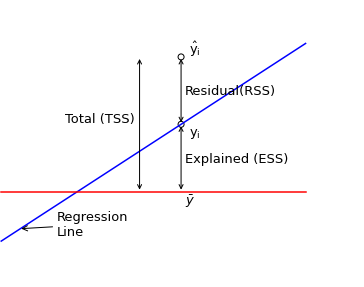
\includegraphics[scale=0.75]{Images/Methods/Correlation/R2_Plot.png}
\caption{\centering Graphic representation of TSS, RSS and ESS.}

\vspace{-1cm}
\end{center}
\end{wrapfigure}
\begin{itemize}
  \item $TSS$ or Total sum of squares: the average squared error between the true value $y_{i}$ and the average $\bar y$.
  \item $RSS$ or Residual sum of squares: the average squared error between the true value $y_{i}$ and the predicted value $\hat y_{i}$ (Equation \ref{eqn:RSS}).
  \item $ESS$ or Explained sum of squares: the average squared error between the predicted value $\hat y_{i}$ and the $\bar y$.
\end{itemize}


The most general definition of the coefficient of determination is given by:

\begin{equation}
R^{2} = 1 - \frac{RSS}{TSS} = \frac{ESS}{TSS}.
\end{equation}

In other words, $R^{2}$ being high means that a high percentage of the total variance is the response variable is explained by the model. A baseline model that always predicts $\bar y$ will have a $R^{2}=0$. $R^{2}$ can have values below zero if the predictions are below this baseline.

It must be kept in mind that these measures of correlation only account for linear dependencies between variables, that is, relationships of the form:

\begin{equation}
    Y = \beta_{0}X_{0} + \beta_{1}X_{1} + \dots + \beta_{k}X_{k}.
\end{equation}

We can observe this phenomenon in the following examples of Figure 2.7.

\begin{figure}[h!]
\centering
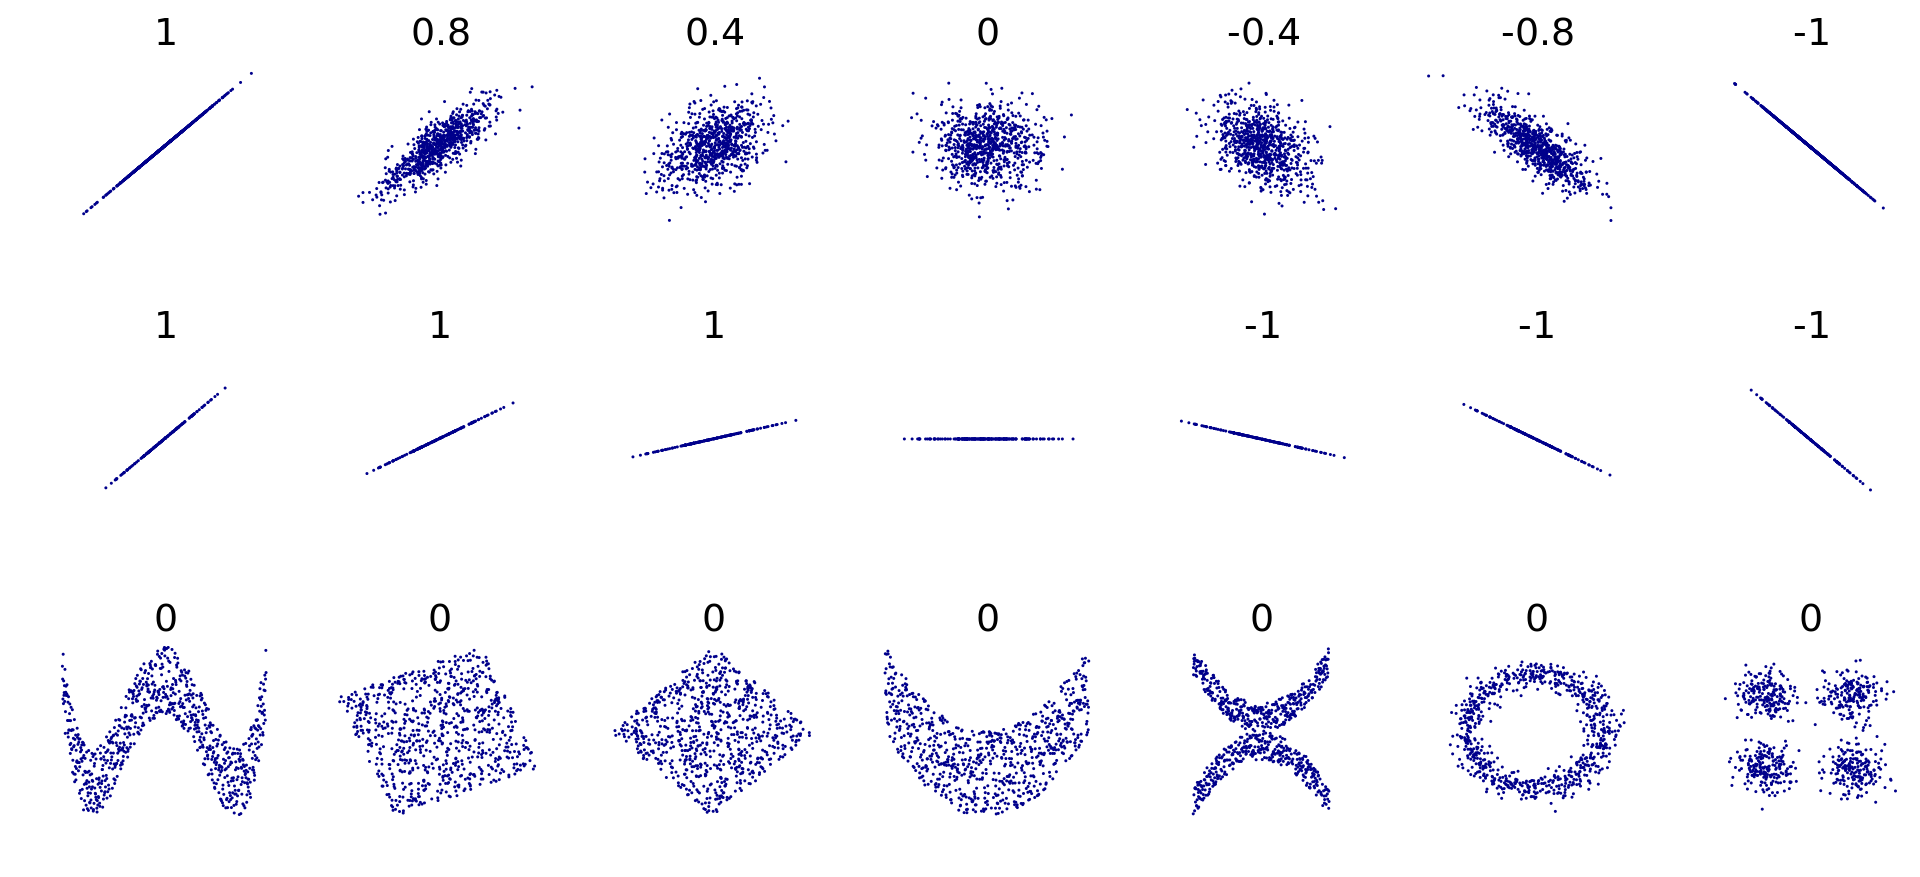
\includegraphics[scale=0.2]{Images/Methods/Correlation/CorrelationValues.png}
\caption{Examples of different R² values.}
\end{figure}    


\subsubsection{Spearman Correlation}
The correlation measures explained above take into account linear dependencies, but do not describe non-linear ones. For this, Spearman's Correlation is defined, which explores the dependencies of the ordinal nature of the given data, rather than the data measure itself. For this, ranks are established, where instead of calculating the correlation of the original variables, the correlation of the ranks of the variables is calculated (Spearman, 1904).  Under the null hypothesis, each rank of X should have the same probability of being associated with each rank of Y. So in Spearman's correlation, it is the covariance between ranks that is taken into account, rather than the covariance between variables. Moreover, as in Pearson's correlation, they are always divided by the respective standard deviations of the ranks:

\begin{equation}
    \rho_s(X,Y)=\frac{\sum(R(x)-N/2)(R(y)-N/2)}{(N-1)\sigma_{R(x)}\sigma_{R(y)}}=\frac{Cov(R(X),R(Y))}{\sigma_{R(X)}\sigma_{R(Y)}}.
\end{equation}

Otherwise, Spearman's correlation is Pearson's correlation in ranks.

Pearson (1907) criticises the Spearman correlation on the grounds, among others, that since it is designed to reflect the relationship even if the relationship is not linear, it also loses the possibility of being considered a regression parameter even if the underlying relationship is linear \cite{Kolassa2020}.

\subsubsection{Kendall Rank Correlation Coefficient}
Another correlation metric that takes into account the ordinal nature of the data is the Kendall rank correlation coefficient, also known as Kendall's $\tau$. To understand the underlying principle of this correlation metric, concordant and discordant pairs need to be defined. Bivariate observations for which the X and Y values are in the
same order are called concordant; pairs that are not concordant are called discordant.\\

Kendall's $\tau$ builds a new calculation which is based on the 
counts of concordant and discordant pairs. The concordant pair number U:
\begin{equation}
    U=\sum_{i<j}^NZ_{ij},
\end{equation}
where\\
\begin{equation}
    Z_{ij}=
    \begin{cases}
    1,\hspace{1.2cm} (X_j-X_i)\cdot(Y_j-Y_i)>0\\ 
    0,\hspace{1.2cm} (X_j-X_i)\cdot(Y_j-Y_i)<0
    \end{cases}.
\end{equation}

Therefore, Kendall's $\tau$ is evaluated subtracting the number of discordant pairs from U, the number of concordant pairs, and then dividing this by the number of ways to choose two items from n items, ${n \choose 2}=n(n-1)/2$ :
\begin{equation}
    \tau= \frac{U-\left({n\choose2}-U\right)}{{n\choose2}}=\frac{4U}{n(n-1)}-1.
\end{equation}\hspace{15cm}\cite{Kolassa2020}
\subsection{Feature Evaluation Metric}
Evaluation of the features themselves is an important part of the machine learning problems.  
In Section 2.2.4, the sequential feature selection algorithm was explained, as well as the reason for its implementation. These models which were worked on implement the feature evaluation metric explained below: F Score.
\subsubsection{F Score}
F Score is a useful and simple evaluation metric specially used for features, where the Pearson correlation between the response and descriptor features is calculated one by one.\\

The descriptors with highest correlation with the response feature are determined to be the ones that have valuable information referring to the response feature, and they therefore have higher scores. 


\section{Model Evaluation}
The process of evaluating whether the model is good or bad enough can be harsh. Feedback in the data used for training the algorithm, such as RSS (or other metrics) that was minimised, does not always provide a full sight of the righteousness of the model; data which is influential in the building of the model does not supply a valuable enough response on whether it will work on raw, virgin data. Therefore, to be able to evaluate afterwards, the data itself has to be separated in a \textbf{training set}, which is used to feed the algorithm; and \textbf{test set}, which is used one and only for the appraisal of the model built. 
\subsection{Learning Curves}
Using learning curves, plenty can be learnt from a model. Inspecting the shape of these can show whether a model is overfit or underfit, depending on the variable chosen. Two curves are set, the test error curve and the training error curve. The test error is the average error that results from using the test set. It is obvious that given a dataset, the use of a particular statistical learning method is warranted if it results in a low test error. The training error is the error obtained in the training set. A low training error with a high test error is a clear result of overfitting (Figure 2.6), while the opposite, a relatively high training error with a lower test error is subject to underfitting (Figure 2.7).
\begin{figure}[h!]
  \centering
  \begin{minipage}[b]{0.45\textwidth}
    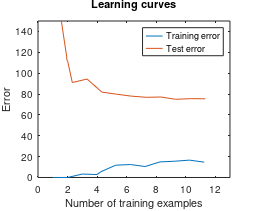
\includegraphics[width=\textwidth]{Images/Methods/Evaluation/overlc.png}
    \caption{Overfitting model.}
  \end{minipage}
  \hfill
  \begin{minipage}[b]{0.45\textwidth}
    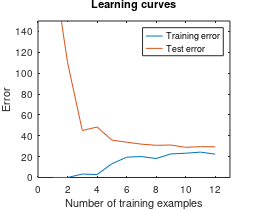
\includegraphics[width=\textwidth]{Images/Methods/Evaluation/goodlc.png}
    \caption{Underfitting model.}
  \end{minipage}
\end{figure}\\

Learning curves can be used for hyperparameter tuning because the optimal hyperparameter value can be chosen to fit neither too well nor too poorly, with as little training and testing error as possible. They can also be plotted as a function of the size of the training set, as in Figures 2.8 and 2.9. These types of learning curves can also show whether the current model is underfitting or overfitting, as well as the potential performance of the model when trained with a larger dataset, since the evolution of these curves as more training examples are added can be predicted by simple observation.

\subsection{Cross-Validation}
The test error can be easily calculated if a specific 
test set is available. Unfortunately, this is usually not the case. In contrast, the training error can be easily calculated by applying the statistical learning method to the observations used in training. The training error rate is often significantly different from the test error rate, and in particular the training error rate can drastically underestimate the test error rate.
\subsubsection{K-Fold Cross-Validation}
K times repeated k-fold cross-validation is commonly used to evaluate the predicted
performance on different predicted models \cite{YUAN2022100026}. In this form of cross-validation, switching portions of data are used to train and to test the models k times.\\

 Figure 2.10 shows a more visual representation of the process. 
\begin{figure}[h!]
    \centering
    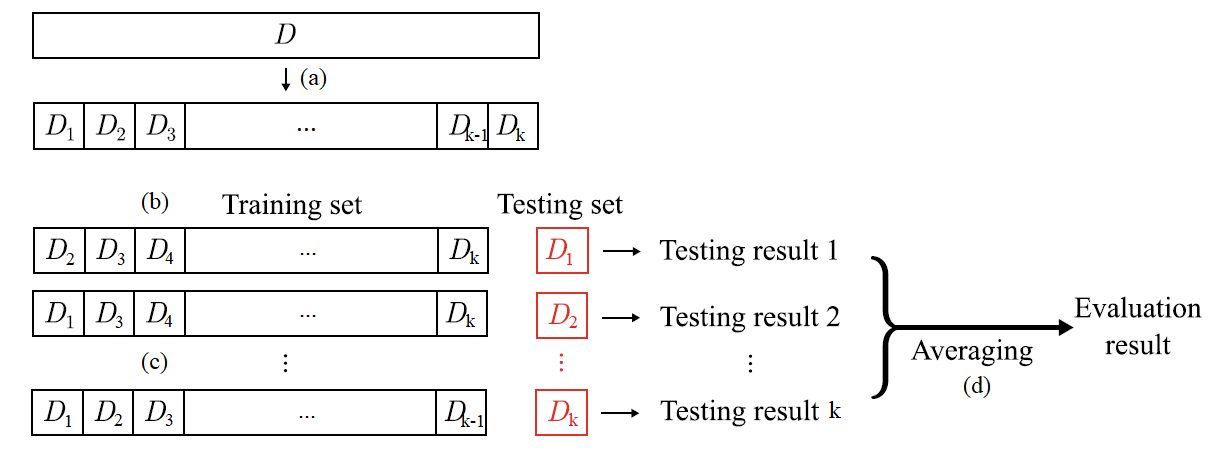
\includegraphics[width=0.7\textwidth]{Images/Methods/CV/Kfcv.png}
    \caption{K-fold cross-validation process. The dataset is broken down in k different subsets, with roughly the same size (a). K-1 subsets are used as training sets, for the algorithm to train itself on, while the remaining subset is used for test (b). The error obtained in this test subset is noted. This process is carried on k times, using each subset as test only once (c), and the mean value of the error is obtained by averaging (d), providing a more precise estimation for the error \cite{Zhou21a}.}
\end{figure}

\subsection{Bootstrapping}
When having used a dataset of size D, the previous method does not offer a chance to evaluate a method trained on D observations, simply because part of these D observations are spared in order to serve as testing virgin data. This provokes an unavoidable estimation bias, specially in the case of smaller datasets, where sparing one observation alone can be able to overthrow the estimation. For these cases, $bootstrapping$ is a solution.\\

In bootstrapping, a new dataset is created, and D observations from the original dataset are randomly put in the new dataset. Sampling without replacement is the way to go, as the same observation can be repeatedly be copied. In this way, we can create a new bunch of same size and different datasets which can be very useful to train and evaluate the model (not reducing the training set size).

\subsubsection{Confidence interval}
Another thing that can be done when wanting to calculate the mean value of the observations, is plotting a histogram of the mean values obtained in each dataset. The more the new datasets, the better the understanding of the actual mean value and its error. This way, we can create intervals in the histogram that encompass a different amount of confidence, and are subsequently called confidence intervals. An 80\% confidence interval, for example, would include 80\% of the mean values calculated through the different datasets (original and new). 

\subsection{Nested Cross-Validation}
A more efficient but computationally expensive evaluation method is nested cross-validation, where a combination of k-fold cross-validations and bootstrapping allows for a more accurate and reliable estimation of the performance. This is why this was the performance guideline evaluation method used in this problem.\\

In nested cross-validation (see Figure 2.11) , 10-fold cross-validation is carried on where training and test sets are generated from the data, this is called the $outer$ $loop$. This training sets are then separated into training and validation sets using 5-fold cross-validation on which is determined to be the $inner$ $loop$. The training sets are used to train the model, utilising the feature selection algorithm, and grid search is used to determine which hyperparameter values fit the model with least error, for these last two, the validation set mentioned beforehand is used.\\\\ 
--------------------------------------------------------------------------------------------------------------------
\subsubsection{Grid Search}
Grid search is used to find the optimal hyperparameter value in the model for the selected dataset. The model is trained with the training set for different hyperparameter values, and the error is calculated for the validation set in each combination.\\

For this, after the learning curve is plotted, it usually happens that it is not clear which value to set as the optimal one. The goal of grid search is to search among a value stretch to choose the one which minimises the error in the validation set. The stretch selected is divided in the selected number $n$, and the different $n$ values are tested.\\

For example, imagine it is not clear which values for number of trees from 0 to 100 and maximum depth of the trees from 2 to 5 best fit the dataset in Random Forest regression.
$n_1$=21 and $n_2$=4 can be chosen, and the values tested would be: 0,5,10,15,20,...,95,100, for number of trees; and 2,3,4,5, for the maximum depth of these trees.
94 (21x4) individual combinations can be tested, the validation set is meant to select the optimal one in the metric chosen.\\\\
\begin{wrapfigure}{r}{0.6\textwidth}
\begin{center}
\vspace{-1.7cm}
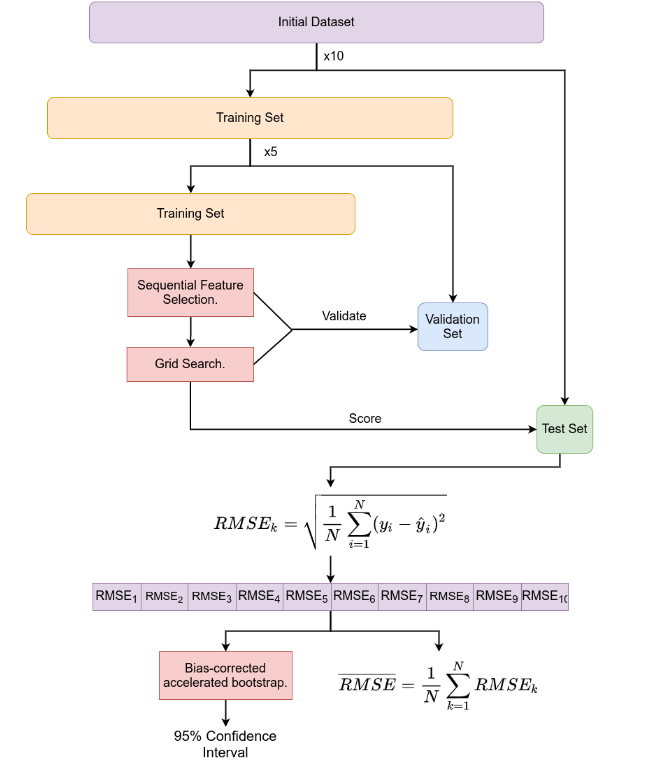
\includegraphics[width=0.6\textwidth]{Images/Methods/CV/Nested CV.png}
\caption{\centering Nested cross-validation diagram.}
\vspace{-1cm}
\end{center}
\end{wrapfigure}
---------------------------------------------\\


The outer test set is used now for the first time. A virgin dataset is needed (validation set was used in grid search and feature selection) to calculate the metric wanted to be determined (RMSE in Figure 2.11) without the influence on which the model was optimised.\\

 With the 10 values obtained (for each fold), on the one hand, a mean value is calculated; on the other hand, bootstrapping is applied to get a 95\% confidence interval. Also, the minimum and maximum values among the 10 values are noted.

\subsection{Reliability}
The reliability of the model is very important after having optimised the algorithm. Comparing hypotheses or models is what is usually done to get a frame of reference of the quality and reliability of the algorithm.   
\subsubsection{Paired Sample T-Test} 
When dealing with two models' results and wanting to compare them, the paired sample t-test provides a viewpoint for when we are concerned about the difference between two variables surrounding the same subject.
This is the formula for the t statistic:
\begin{equation}
    t=\frac{\overline{x_1}-\overline{x_2}}{\sqrt{\frac{\sigma_1}{n_1}+\frac{\sigma_2}{n_2}}},
\end{equation}
where $\overline{x}$ is the mean value for the variable, $\sigma$ is the standard deviation and n accounts for the data points. The suffixes 1 and 2 refer to each hypothesis tested.
\subsubsection{Empirical p-values}
P-values define the probability that a t statistic, or higher, would be obtained from the t distribution.\\

The percentage of error that we are willing to run our test with each one of the hypothesis is the significance $\alpha$. It can be set to whichever value wanted, but the most usual is 0.05, equivalent to 5\%, for hypothesis testing. Consequently, a p-value smaller than $\alpha$ discards the equivalence \cite{pvalue}. 
 

 












